\pdfminorversion=4
\documentclass[aspectratio=169]{beamer}
\usepackage{animate} % for animation
\usepackage{array,multirow,graphicx}
\usepackage{multicol}
\usepackage{etoolbox}

\graphicspath{{/home/fafaa/Documents/sinyal_dan_sistem/Slide/gambar}
               {/home/fafaa/Pictures}}
\setbeamertemplate{caption}[numbered]
\setbeamertemplate{section in toc}[sections numbered]

% Hide subsubsections from TOC, but keep PDF bookmarks with beamer
\hypersetup{bookmarksopen=true,bookmarksopenlevel=4}
\setcounter{tocdepth}{4}

\renewcommand{\figurename}{Gambar.}
\renewcommand{\tablename}{Tabel.}

\usetheme[pageofpages=of,	% String used between the current page and the
							% total page count.
			alternativetitlepage=true,% Use the fancy title page.
			titleline=true,
			titlepagelogo=OK-LOGO-ITK.jpg
%          	 titlepagelogo=fig/jaist_logo.png
			]{Torino}
			% change /beamerinnerthemefancy.sty to resize the logo
\usecolortheme{freewilly}

\makeatletter
\patchcmd{\beamer@sectionintoc}{\vskip1.5em}{\vskip0em}{}{}
\makeatother

\author{Mifta Nur Farid \\
	miftanurfarid@lecturer.itk.ac.id}
\title{Sinyal dan Sistem}
\subtitle{Pengantar Sinyal \& Sistem}
\institute{Teknik Elektro \\ Institut Teknologi Kalimantan \\ Balikpapan, Indonesia}
\date{\tiny Februari 26, 2020}

% The log drawn in the upper right corner.
\logo{
\includegraphics[height=0.13\paperheight]{OK-LOGO-ITK.jpg}}

\begin{document}

\begin{frame}[t,plain]
\titlepage
\end{frame}

\section{Sinyal}

\begin{frame}{Sinyal}
	\begin{itemize}
		\item Sinyal direpresentasikan secara matematis sebagai fungsi dari satu atau lebih variabel bebas
	\end{itemize}
	\begin{multicols}{2}
		\begin{figure}
			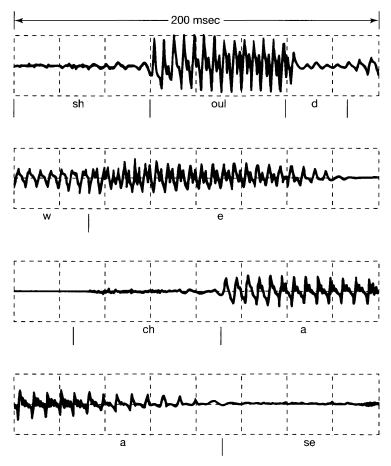
\includegraphics[width=0.5\linewidth]{00.sinyal_suara}
			\caption{Sinyal suara, 1 variabel (tekanan suara terhadap waktu), \textit{one-dimensional}}
		\end{figure}
		\begin{figure}
			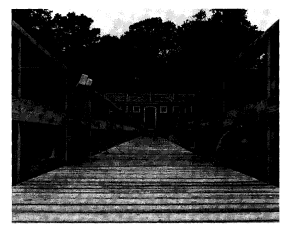
\includegraphics[width=0.7\linewidth]{00.sinyal_gambar}
			\caption{Gambar, 2 variabel (brightness terhadap sumbu vertikal dan horizontal), \textit{two-dimensional}}
		\end{figure}
	\end{multicols}
\end{frame}

\begin{frame}{Sinyal waktu diskret dan kontinu}
	\begin{multicols}{2}
		\begin{itemize}
			\item Sinyal waktu diskrit
			\begin{itemize}
				\item Variabel bebasnya bernilai diskret
				\item Dinotasikan dengan $ x[n] $
				\item $ n $ adalah variabel bebas dengan bilangan bulat
				\item Jika ada 2 variabel bebas $ \rightarrow ~ x[m,n] $ , dst.
			\end{itemize}
			\item Sinyal waktu kontinu
			\begin{itemize}
				\item Variabel bebasnya bernilai kontinu
				\item Dinotasikan dengan $ x(t) $
				\item $ t $ adalah variabel bebas
				\item Jika ada 2 variabel bebas $ \rightarrow ~ x(t,s) $, dst.
			\end{itemize}
		\end{itemize}
		\vfill\null
		\columnbreak
		\begin{figure}
			\centering
			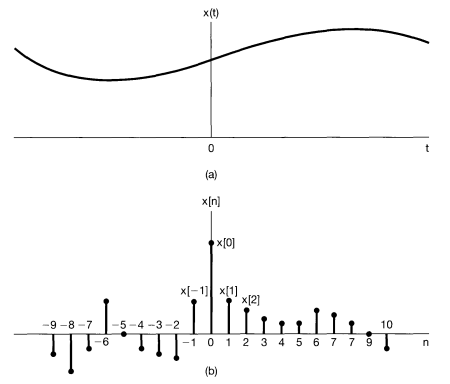
\includegraphics[height=0.65\textheight]{00.representasi_grafis_dari_sinyal_waktu_kontinu_dan_diskret}
			\caption{Representasi grafis dari sinyal waktu kontinu dan diskret}
		\end{figure}
	\end{multicols}
\end{frame}

\begin{frame}{Contoh sinyal waktu diskret}
	\begin{figure}
		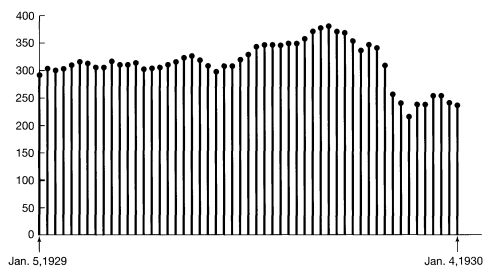
\includegraphics[height=0.7\textheight]{00.sinyal_waktu_diskret}
		\caption{Grafik \textit{stock market index} adalah contoh sinyal waktu diskret}
	\end{figure}
\end{frame}

\begin{frame}{Contoh sinyal waktu kontinu}

	\begin{figure}
		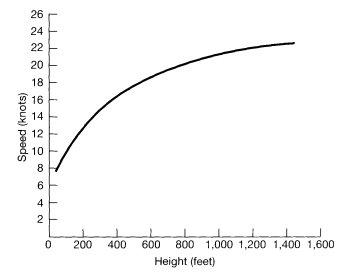
\includegraphics[height=0.7\textheight]{00.sinyal_waktu_kontinu}
		\caption{Grafik profil kecepatan angin adalah contoh sinyal waktu kontinu}
	\end{figure}
\end{frame}


\section{Sistem}

\begin{frame}{Sistem}
	\begin{multicols}{2}
		\begin{itemize}
			\item Sistem berfungsi untuk memproses sinyal
			\item Sistem linear / non-linear
			\item Sistem time-invariant / time-varying
			\item Fokus kita nantinya di linear time-invariant (LTI)
		\end{itemize}
		\vfill\null
		\columnbreak
		\begin{figure}
			\centering
			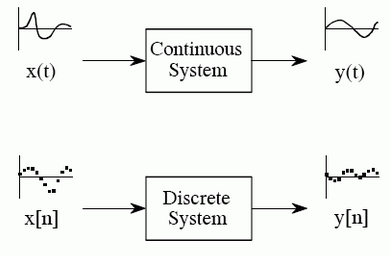
\includegraphics[height=0.5 \textheight]{gambar/00.sistem}
			\caption{Terminologi sinyal dan sistem}
		\end{figure}
	\end{multicols}
\end{frame}

\begin{frame}{Contoh sistem diskret}
	\begin{figure}
		\centering
		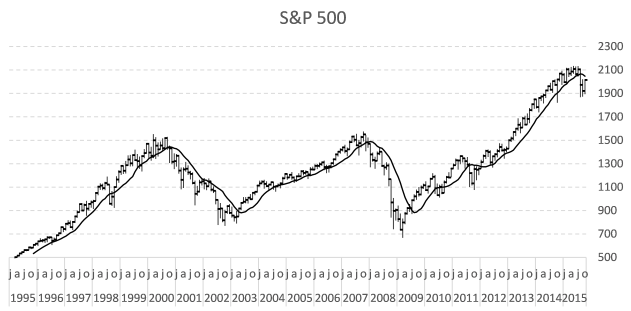
\includegraphics[height=0.7\textheight]{gambar/00.proses_sinyal_diskret}
		\caption{Market trend}
	\end{figure}
\end{frame}

\begin{frame}{Contoh sistem kontinu}
	\begin{figure}
		\centering
		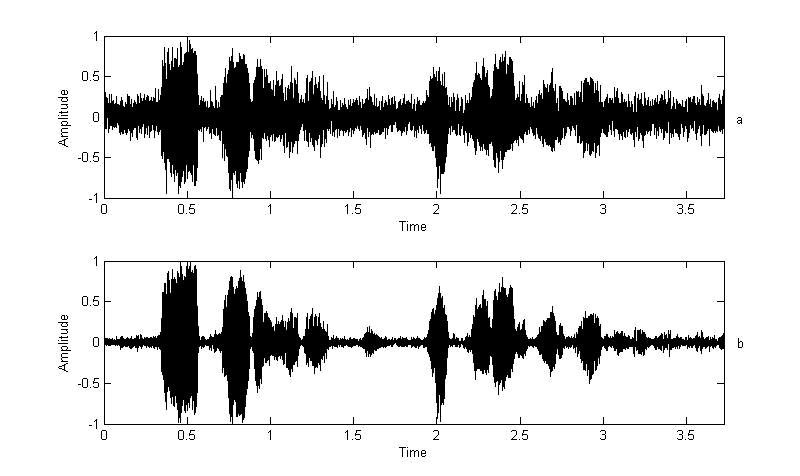
\includegraphics[height=0.7\textheight]{gambar/00.proses_sinyal_kontinu}
		\caption{Menghilangkan noise dari suara rekaman (gambar atas = suara dengan noise, gambar bawah = noise sudah dihilangkan)}
	\end{figure}
\end{frame}

\begin{frame}{Contoh sistem yang memproses sinyal multi-dimensional}
	\begin{multicols}{2}
		\begin{figure}
			\centering
			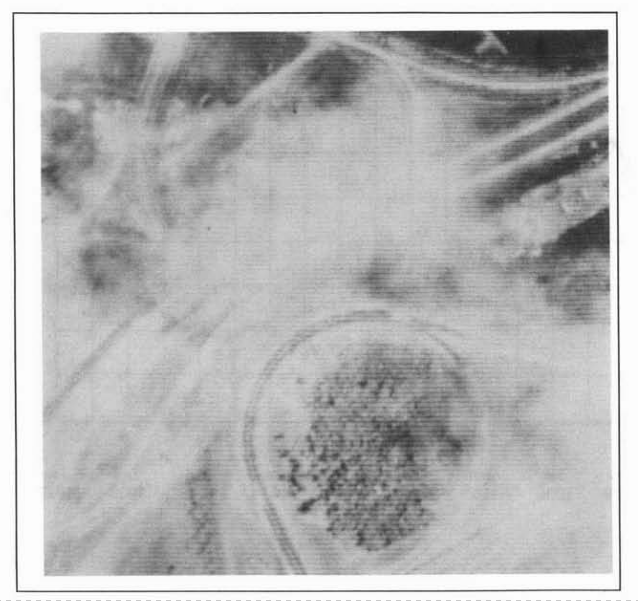
\includegraphics[height=0.65\textheight]{gambar/00.foto_jalan_berawan}
			\caption{Foto jalan berawan}
		\end{figure}
		\vfill\null
		\columnbreak
		\begin{figure}
			\centering
			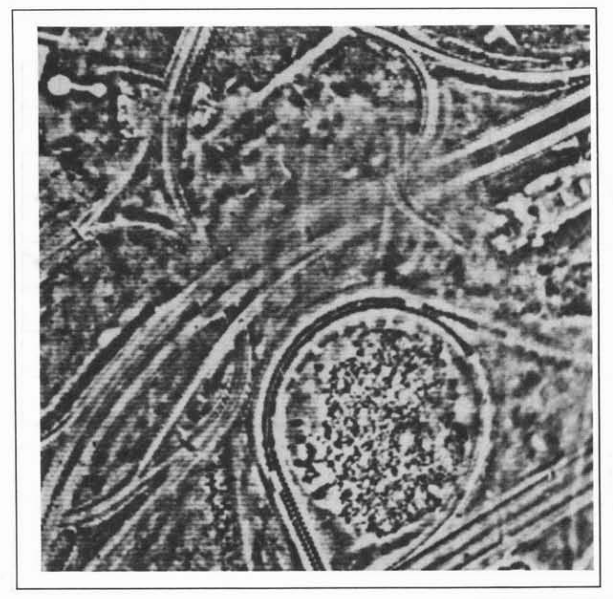
\includegraphics[height=0.65\textheight]{gambar/00.foto_jalan_awan_hilang}
			\caption{Hasil pemrosesan menghilangkan awan}
		\end{figure}
	\end{multicols}
\end{frame}
\begin{frame}{Interkoneksi antar sistem}
	\begin{itemize}
		\item Terkadang antara satu sistem dengan sistem lainnya saling terinterkoneksi
		\item Interkoneksi antar sistem :
		\begin{enumerate}
			\item Seri
			\item Paralel
			\item \textit{Cascade} (Bertingkat)
			\item \textit{Feedback} (Umpan-balik) $ \leftarrow $ akan menjadi topik utama dalam kuliah ini
		\end{enumerate}
	\end{itemize}
\end{frame}

\begin{frame}{\textit{Domain} (ranah) dalam analisis dan representasi}
	\begin{multicols}{2}
		\vfil\null
		\begin{enumerate}
			\item \textit{Time-domain} (ranah waktu)
			\begin{itemize}
				\item $ x(t) $
				\item $ x[n] $
			\end{itemize}
			\item \textit{Frequency-domain} (ranah frekuensi)
			\begin{itemize}
				\item \textit{Fourier transform}
				\item \textit{Laplace transform}
				\item \textit{$ \mathcal{Z} $-Transform}
			\end{itemize}
		\end{enumerate}
		\vfil\null
		\columnbreak
		\begin{figure}
			\centering
			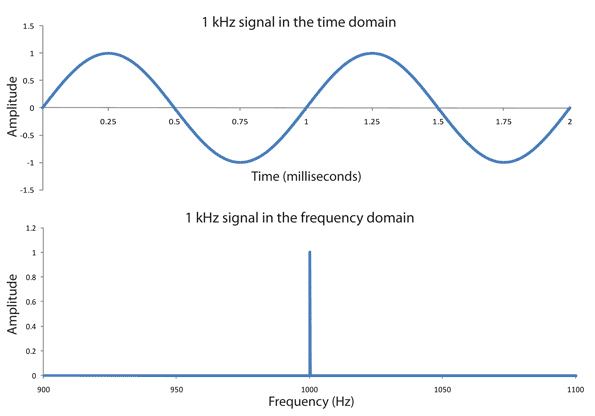
\includegraphics[height=0.6\textheight]{gambar/00.TimeDomain}
			\caption{Contoh sinyal ranah waktu (atas) dan ranah frekuensi (bawah)}
		\end{figure}
	\end{multicols}
\end{frame}
\end{document}

